\chapter{Change-Point Analysis in language development: a study of voice onset time production in a multilingual system}\label{ch:adrielledecar3}
\chapterauthor[1,2]{Laura Castilhos Schereschewsky}
\chapterauthor[1,3]{Ubiratã Kickhöfel Alves}
\begin{affils}
\chapteraffil[1]{Universidade Federal do Rio Grande do Sul}
\chapteraffil[2]{CAPES}
\chapteraffil[3]{CNPq}
\end{affils}

%%%%%%%%%%%%%%%%%%%%%%%%%%%%%%%%%%%%%%%%%%%%%%%%%%%%%%%%%%%%%%%%%%%%%%
\section{Introduction}


According to Complex Dynamic Systems Theory (CDST) \citep{larsen-freeman2008,lowie2015,lowie2019},
when it comes to
multilingual development, we need to think about the interconnectedness of the
system components. Departing from this assumption, we follow Kupske's concept
of language attrition\footnote{In this paper, we do not differentiate ‘language
attrition’ from ‘language transfer’ or ‘language drift’. We will use the three
terms interchangeably.}, which characterizes this phenomenon as the force
resulting from the contact of two bodies, in this case, two languages, that are
in constant movement \citep[p.~39--40]{kupske2016}. This concept embraces the
CDST premise that change is inherent to development. Thus, if the system is in
constant movement, we may find it in continuous change in a given state, and
language variability is expected to be found. Sometimes, the system may go
through significant changes that exceed its current state \citep{van_dijk2007}.
If these particular changes lead to the reorganization of the
system as a whole (as in the emergence of a new attractor state), we call them
‘phase transitions’ or ‘phase shifts’. According to \citet{hepford2020}, this new
attractor state is not necessarily something new to learners, as it "could be a
language form that they are exposed to regularly but have not had the cognitive
ability to adapt to, or an event that pushes a learner to adapt and
self-organize resulting in using a new form" \citep[p.~162--163]{hepford2020}.

Based on the aforementioned assumptions, this study aims to investigate the
phenomena that occur in the development of the additional languages of
trilingual speakers, native speakers of Brazilian Portuguese (BP-L1) and
non-native speakers of English (L2) and French (L3). Specifically, this
longitudinal study analyzes, over a period of three months (with 12 weekly
datapoints), the development of the production of Voice Onset Time (VOT),
observing possible phase shifts through change-point analyses \citep[cf.]{taylorwayne}
provided by the Change-point analyzer v.2.3 software \citep{taylor-analyzer}. 
The study included a period of pedagogical intervention to accelerate
the development of the positive VOT pattern with the characteristic aspiration
of English. This teaching intervention took place over six explicit
pronunciation instruction sessions, conducted in the weeks of datapoints 4 to
9. We aimed to discuss to what extent the accelerated development of an L2 with
a typologically different VOT pattern causes changes in the development of the
L3 and L1 subsystems, as well as show the inter-relation of the two additional
languages over time.

According to the literature \citep[cf.]{schereschewsky2021}, from the study of VOT,
we can observe the multidirectionality of transfer and the adaptability and the
self-organization of language subsystems. Therefore, this study intends to
provide empirical and theoretical input into a larger  understanding of these
aspects. This may shed light on the development of additional languages in the
light of CDST. As this is essentially a theory about change, we aim to raise
issues such as language development and its ongoing "process" in time \citep[cf.]{lowie2015,lowie2019},
the interconnectivity of typologically different
subsystems, data variability, and the emergence of new attractor states and
phase shifts.


%%%%%%%%%%%%%%%%%%%%%%%%%%%%%%%%%%%%%%%%%%%%%%%%%%%%%%%%%%%%%%%%%%%%%%
\section{Method}
As addressed in the previous section, the main goal of this study was to
inferentially verify possible phase shifts in VOT patterns, in each of the
language subsystems, especially after the beginning of explicit pronunciation
instruction in English. For that, we carried out change-point analyses \citep[cf.]{taylorwayne}.

In order to achieve our goal, we proposed a methodology in which changes and
interactions among the subsystems of multilingual speakers could be
investigated through accelerating L2 VOT development. The experiment was built
with a longitudinal design in an A-B-A format \citep[cf.]{hiver2020},
with 12 datapoints, which were intersected in the midpoints with 6 sessions of
explicit pronunciation instruction in English. This intervention took place
between the weeks referring to datapoints 4 and 9, and all instructional
sessions were conducted with a communicative approach.

In this study, we replicated different process-oriented analyses to encompass
and address variability \citep{garcia2013}, conducting the same experiment with
five participants from different backgrounds, different ages, with different
proficiency levels in their additional languages, and different routines. Due
to space restrictions, in this paper we will focus on the results from one
particular participant\footnote{This participant is referred to as Participant
5 in previous works from this project. For more information on the other
participants, see \citet{schereschewsky2021}.}, who was 24 years old at the time, a
graduate student who worked as a French teacher. This participant took a
self-evaluation test \cite{schereschewsky2021}%\citep{scholl2013}%(SCHOLL; FINGER, 2013) 
and graded herself a 6 in English
and a 10 in French\footnote{It is interesting to note that her L3 was more
active than her L2, because she worked as a French teacher, even though she had
started studying English before she even started learning French.}.

The participant was presented with three different reading tasks. In each data
collection session, she received 23 carrier sentences (repeated three times
each) with 18 target words with /p/, /t/ and /k/ in word-initial position and 5
distractor words. The BP and English instruments were the same as in Kupske
(2016), for both matters of consistency and comparisons of results with
previous studies. We also used the same methodological control as Kupske in the
development of the French instrument \citep[cf.]{schereschewsky2021}. Because she
received the same target words, the order of the carrier sentences was
randomized and the distractor words were changed each week. This study was
conducted during the pandemic of COVID-19, so the participant accomplished the
experiment in an individual setting and was asked to complete each task taking
time intervals between them.

All audio recordings from the reading tasks were analyzed acoustically in the
Praat v.6.1.16 software \citep{boersma2019}. Due to time and space
restrictions, only the absolute values of VOT production were considered. As
for VOT measurements, similar criteria to previous works were used: selecting
the voiceless interval between the burst of the stop consonant and the first
regular pulse of the following vowel.

As for the statistical analyses, the participants' developmental trajectories
were plotted, considering minimum, maximum, and mean values from the tokens of
each stop consonant in each datapoint. Following that, change-point analyses
\citep[cf.]{taylorwayne,steenbeek2012,baba2014,han2018,englhardt2020,henry2021}
were conducted. Change-point analysis is an inferential method that uses resampling
and cumulative sums to identify a pattern shift, or the point of change, in a
set of longitudinal data.

The Change-Point Analyzer software is able to detect several longitudinal
changes. By running a fast analysis of cumulative sums and bootstrapping, for
each change in pattern, the software provides practical information, including
the confidence level, which indicates a probability that a change has actually
occurred, and the confidence interval, which indicates when that change has
occurred. Figure 1 shows the first output tab from the software, with the
change-point analysis visual plot.

\begin{figure}[h]
\centering
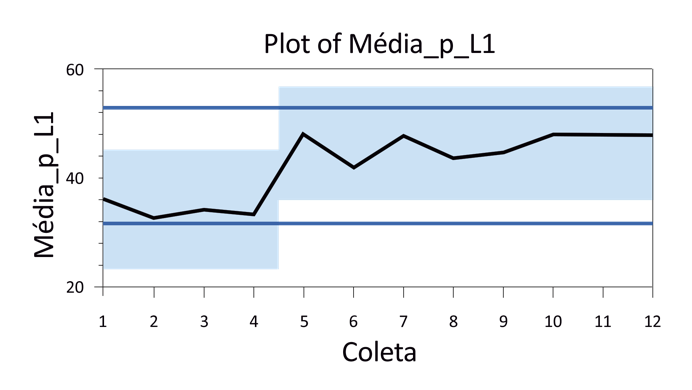
\includegraphics[width=0.7\linewidth]{imgs/lauracastilho22-image1.png}
\caption{Outputs - change-point analysis visual plot.} 
\label{laura-fig01}
\end{figure}

In Figure \ref{laura-fig01}, the bold black line in the graph represents the raw data of the
mean VOT values of [p] in Participant 5’s L1 over the 12 collection points. The
dark blue lines represent the amplitude range of the control limits, that is,
the maximum range of variation in which the values can fluctuate, assuming that
no change has occurred (if the black line exceeds the control limits, we will
have a first indicative that a change has taken place, which may simply be an
outlier or an indication of an actual phase shift). The lighter blue background
represents the area that should contain all values varying within the control
limits. The displacement of this area in light blue at the bottom of the graph
actually indicates a phase shift, as the average values within the first
segment show a sudden change, starting to vary in a different range,
represented by the second segment of the area in lighter blue. Figure \ref{laura-fig02} shows
the second output tab from the software, with the significant changes of the
set of data.

\begin{figure}[h]
\centering

\includegraphics[width=\linewidth]{imgs/lauracastilho22-image2.png}
\caption{Outputs - table of significant changes.} 
\label{laura-fig02}
\end{figure}

The table in Figure \ref{laura-fig02} indicates the estimated point of change to another phase,
in this case, in Datapoint \#5, with a confidence level of 97\%\footnote{The
Change-point Analyzer only presents, in the outputs, intervals that have at
least 95\% confidence. The more spaced the confidence interval, the lower the
confidence level for a change to have occurred at the point identified by the
software.}, indicated by the confidence interval (which, in this case, points
exactly to session 5). Next, the table indicates the values before and after
the change, that is, the average values of variation in the first phase
(considering the average of all inputs within this first phase), which go from
34.25ms to 46.29ms in the second phase. Finally, the level of change indicates
its importance. In this particular example, the Level 1 change indicates that
this was the first significant change identified by the software in the first
analysis run of the data. Other change levels may appear, depending on how many
phase changes are identified and whether these are significant. Finally, Figure
\ref{laura-fig03} shows the third output tab from the software, with the visual chart showing
the cumulative sums.

\begin{figure}[h]
\centering
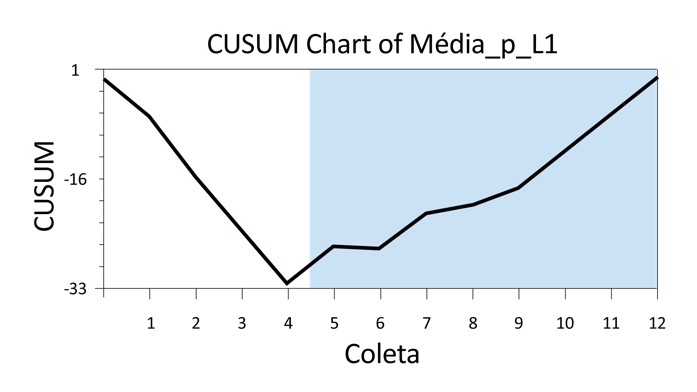
\includegraphics[width=0.7\linewidth]{imgs/lauracastilho22-image3.png}
\caption{Outputs - table of significant changes.} 
\label{laura-fig03}
\end{figure}

The chart in Figure \ref{laura-fig03} represents the cumulative sum analyses (CUSUM).
According to \citet[p.~6]{taylorwayne}, "they are the cumulative sums of differences
between the values and the average". These differences sum to zero so the
cumulative sum always ends at zero. Thus, in the CUSUM graph from this data, a
downward sloping line can be seen, indicating that the values in that period
have a tendency to be below the general average, until there is a change in the
direction of the line, starting to have an upward slope, indicating that values
from that portion of the graph tend to be above the overall mean. We should
also look at the shaded background of the chart, which indicates whether and
where there has been a significant change in the slope of the line, referring
to the table with confidence intervals. Another important information brought
by the CUSUM chart is that the straighter the line, regardless of its direction
(up or down), the greater the certainty that no change occurred in that period.
On the other hand, the more curved the line is, as is the case between points 4
and 9, the greater the possibility that other changes (from other levels) have
taken place.


%%%%%%%%%%%%%%%%%%%%%%%%%%%%%%%%%%%%%%%%%%%%%%%%%%%%%%%%%%%%%%%%%%%%%%
\section{Results}

As previously mentioned, change-point analyses are used to identify the points
at which a pattern change occurs in a longitudinal dataset. Thus, change-point
analyses help identify the developmental stages of VOT production, checking
attractor states in phases of relative stability in each language. In this
section, only a summary of the significant changes and the most relevant charts
for the discussion will be presented. A table will presented for each language,
with the significant results split by consonant (/p, t, k/), of the data
collection session the change took place, the confidence interval, the
confidence level (in percentages), the mean values before and after the change
(which is related to the averages of variation of values within the control
limits of each phase) and the level of change (degree of importance in the
analysis by the software). Table 1 shows the results of Brazilian
Portuguese-L1.

\begin{table}[h]
\caption{Change-point analysis of BP-L1.}\label{laura-table01}
\begin{tabular}{@{}lllllll@{}}
\toprule
\textbf{Stop} & \textbf{Measure} & \textbf{Session} & \textbf{Conf.level} & \textbf{From} & \textbf{To} & \textbf{Shift} \\
\midrule
{[}p{]} & Mean & 5 & 97\% & 34,252 & 46,289 & ↗ \\
{[}p{]} & Max & 5 & 95\% & 69,097 & 84,571 & ↗ \\
{[}t{]} & Mean & 11 & 100\% & 40,181 & 32,775 & ↘ \\
{[}t{]} & Max & 11 & 99\% & 76,253 & 48,585 & ↘ \\
{[}k{]} & Mean & 4 & 96\% & 59,073 & 75,531 & ↗ \\
\bottomrule
\end{tabular}
\end{table}

First, we emphasize the interconnectedness of the language subsystems, which
makes it possible for a native language to change, even if it is typologically
different from a language that underwent an intervention, as we found
significant phase changes in the production of VOT in Portuguese-L1 in the
three stops.

For [p], we found a Level 1 phase shift in the means in Datapoint 5, when the
averages change from 34.25ms to 46.29ms, and a Level 3 change in maximums
around Datapoint 5, when the averages increase from 69.1ms to 84.57ms.

For [t], in which we also found significant phase changes in the averages and
maximum instances, the data are somewhat more interesting. In both measures,
Level 2 phase changes are found, in which the VOT decreases in duration. For
the means, phases shifted from an average of 40.18ms to 32.78ms. For the
maximum instances, they shifted from 76.25ms to 48.59ms. However, as both
changes are Level 2 and this new phase with shorter VOT measures only starts by
the end of the analyzed period, around Datapoint 11, it is also necessary to
visually analyze these data, since there is also the possibility that another
(non-significant) change occurred in previous datapoints. Figure
\ref{laura-fig04} shows the change-point analysis plots for the two measures.

\begin{figure}[h]
\centering
\subfloat[\label{laura-fig04-1}]{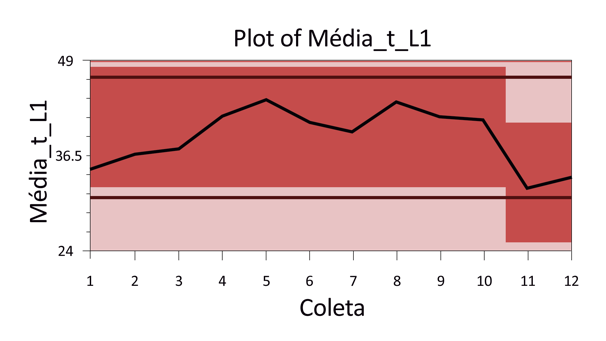
\includegraphics[width=0.45\textwidth]{imgs/lauracastilho22-image4.png}} \qquad
\subfloat[\label{laura-fig04-2}]{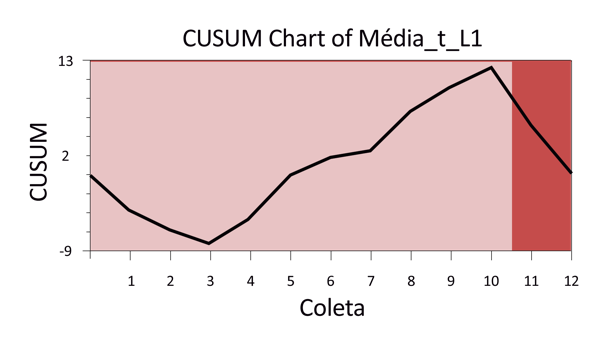
\includegraphics[width=0.45\textwidth]{imgs/lauracastilho22-image5.png}} \\
\subfloat[\label{laura-fig04-3}]{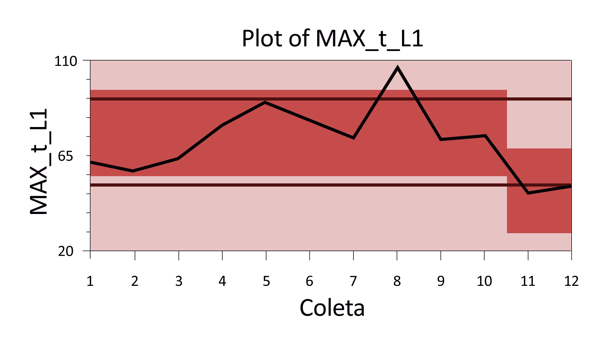
\includegraphics[width=0.45\textwidth]{imgs/lauracastilho22-image6.png}} \qquad
\subfloat[\label{laura-fig04-4}]{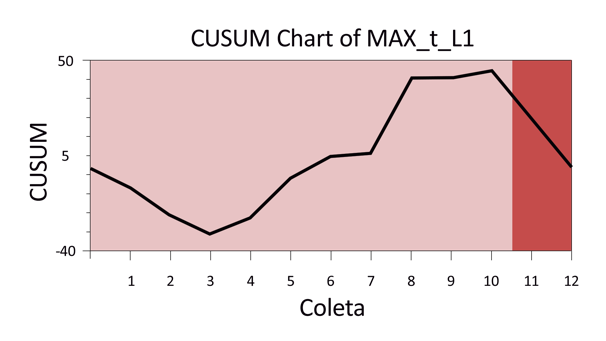
\includegraphics[width=0.45\textwidth]{imgs/lauracastilho22-image7.png}} 
\caption{Change-point analysis of means and maximum instances of [t] in Portuguese-L1.}
\label{laura-fig04}
\end{figure}

The graphs of the means and the maximum instances of [t] show that the two
measures presented a very similar behavior during the analyzed period.
Comparing the initial and final points of the measurements, there is a clear
trend towards a decrease in the descriptive values of VOT, which is in
accordance with the phase shift found with a decrease of averages. However,
there is also a very clear indication that the data may have undergone another
phase shift, around Datapoint 3, where the VOT appears to have increased in
duration. The CUSUMs graph shows the possibility of another phase shift due to
the sudden change in the direction of the cumulative sums line on the third
datapoint. However, the software did not verify this change as significant to
include it in the outputs. What was included in the outputs was a significant
Level 1 phase shift in the means of [k], where there was an increase in the
averages from 59.07ms to 75.53ms in Datapoint 4, thus after the beginning of
the intervention, once again showing that even the subsystem of a typologically
different language is subject to change as a result of another one changing.


\begin{table}[h]
\caption{Change-point analysis of English-L2.}\label{laura-table02}
\begin{tabular}{@{}lllllll@{}}
\toprule
\textbf{Stop} & \textbf{Measure} & \textbf{Session} & \textbf{Conf.level} & \textbf{From} & \textbf{To} & \textbf{Shift} \\
\midrule 
{[}p{]} & Mean & 4 & 97\% & 54,553 & 95,416 & ↗ \\
{[}p{]} & Max & 4 & 94\% & 104,37 & 142,81 & ↗ \\
{[}t{]} & Min & 12 & 91\% & 40,409 & 26,24 & ↘ \\
{[}t{]} & Mean & 4 & 94\% & 62,407 & 105,89 & ↗ \\
{[}t{]} & Mean & 11 & 93\% & 105,89 & 80,07 & ↘ \\
{[}t{]} & Max & 4 & 100\% & 110,1 & 147,2 & ↗ \\
{[}k{]} & Mean & 4 & 99\% & 82,73 & 112,96 & ↗ \\
{[}k{]} & Max & 5 & 91\% & 130,65 & 157,73 & ↗ \\
\bottomrule
\end{tabular}
\end{table}

The English-L2 results also bring valuable data to the discussion. For [p],
there is a significant change in Datapoint 4, the first after the start of the
intervention. When it comes to the means, the Level 2 phase shift occurs when
the average changes from 54.55ms to 95.42ms. For the maximums, the Level 1
change occurs with an increase of the averages from a phase of 104.37ms to
142.81, with very high values of VOT production for a bilabial stop.


For [t], we found significant phase changes for the three analyzed measures,
but each measure presented a different result. For minimums, for instance, a
Level 3 phase shift occurs around Datapoint 12, with a decrease in averages
from 40.41ms to 26.24ms. With such a large confidence interval, which covers
the entire intervention until the end of the study, in addition to the fact
that it is a Level 3 change, there remains a possibility of another, less
significant phase shift, in some other datapoint in that interval. For the
means, two significant phase changes were identified, one of Level 1, in
Datapoint 4, with an increase in the averages from 62.40ms to 105.89ms, and one
of Level 2 , at the end of the study, around Datapoint 11, this time with a
decrease in averages (much like what happens in her L1) from 105.89ms to
80.07ms, a higher average than in the initial phase. The maximums of [t]
present a third pattern of behavior, with a Level 3 phase shift around
Datapoint 4, with an increase from 110.1ms to 147.2ms in the later phase.

\begin{figure}[h]
\centering
\subfloat[\label{laura-fig05-1}]{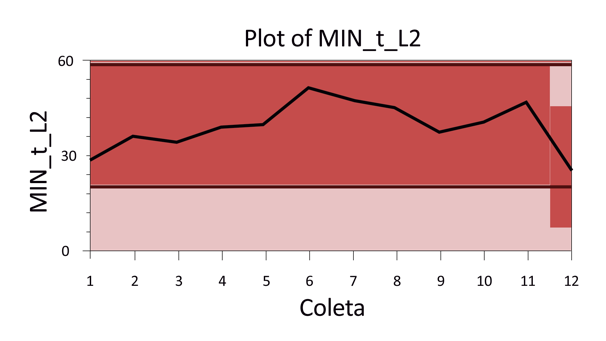
\includegraphics[width=0.45\textwidth]{imgs/lauracastilho22-image8.png}} \qquad
\subfloat[\label{laura-fig05-2}]{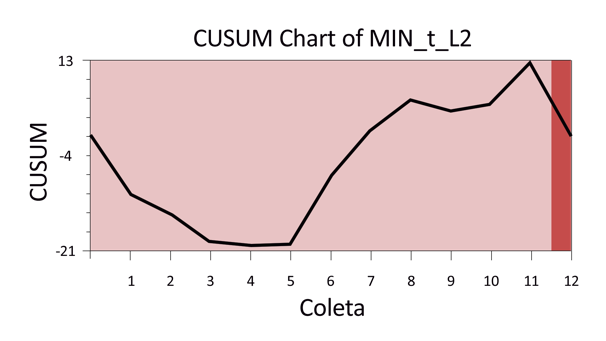
\includegraphics[width=0.45\textwidth]{imgs/lauracastilho22-image9.png}} \\
\subfloat[\label{laura-fig05-3}]{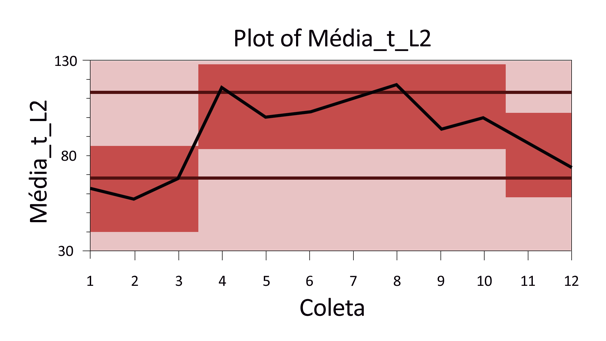
\includegraphics[width=0.45\textwidth]{imgs/lauracastilho22-image10.png}} \qquad
\subfloat[\label{laura-fig05-4}]{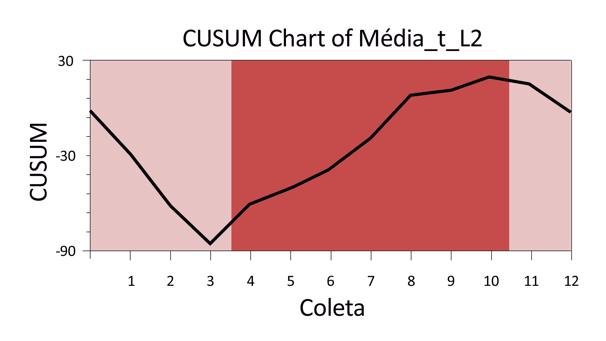
\includegraphics[width=0.45\textwidth]{imgs/lauracastilho22-image11.png}} \\
\subfloat[\label{laura-fig05-5}]{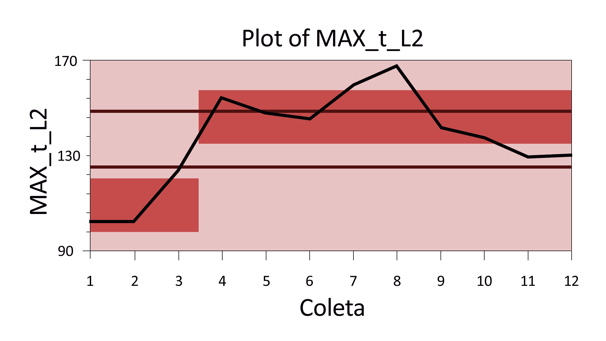
\includegraphics[width=0.45\textwidth]{imgs/lauracastilho22-image12.png}} \qquad
\subfloat[\label{laura-fig05-6}]{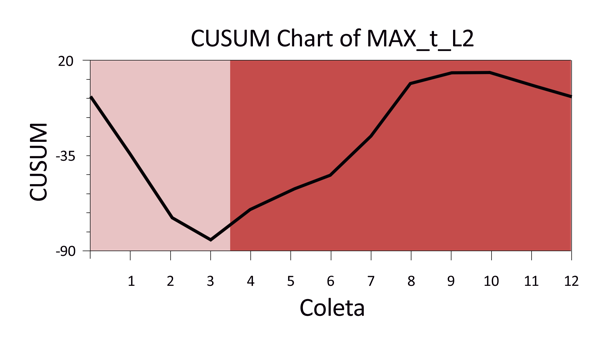
\includegraphics[width=0.45\textwidth]{imgs/lauracastilho22-image13.png}} 
\caption{Change-point analyses of the minimums, means and maximums of [t] in English-L2.}
\label{laura-fig05}
\end{figure}

Figure \ref{laura-fig05} shows the plots of the change-point analyses of the
three analyzed measures of [t] in English-L2. Although the three measures show
completely different behaviors in the outputs, as evidenced by the first graph
of each one, the CUSUM graphs of the three are very similar, indicating sudden
changes in the slope of the cumulatives sums line at least twice on
each\footnote{A downward-sloping CUSUM line indicates values below the overall
average, while an upward-sloping line indicates values above the overall
average. A change in the slope of the line represents a change in trend and,
being a significant change, corresponds to a phase shift.}. This
pattern would be indicative of at least three distinct phases during the study,
in which the first phase change would represent an increase in the average VOT
values, and the second a slight decrease, as we verified in the means of [t],
almost always involving the same datapoints. For minimums and maximums,
however, a possible second phase change was not significant, leaving the
observation only for a qualitative discussion. 

Finally, for [k], we found significant phase shifts in the means and in the
maximums, both indicating an increase in VOT values. For the means, the change
occurred in Datapoint 4, where a new phase went from an average of 82.73ms to
112.96ms. For the maximums, the change occurred around Datapoint 5, when the
results show an increase of the averages from 130.65ms to 157.73ms. Overall,
all these English-L2 data are extremely valuable in showing the influence of
explicit instruction in the development of new attractor states, that is, new
phases developing a non-native positive VOT pattern with long-lag aspiration.
Furthermore, these data highlight change as an inherent characteristic of a
developing system, showing that the language remains in motion even after the
end of an intervention. 

\begin{table}[h]
\caption{Change-point analysis of French-L3.}\label{laura-table03}
\begin{tabular}{@{}lllllll@{}}
\toprule
\textbf{Stop} & \textbf{Measure} & \textbf{Session} & \textbf{Conf.level} & \textbf{From} & \textbf{To} & \textbf{Shift} \\
\midrule 
{[}p{]} & Mean & 4 & 97\% & 30,987 & 40,782 & ↗ \\
{[}p{]} & Max & 4 & 96\% & 60,697 & 78,477 & ↗ \\
{[}t{]} & Mean & 4 & 99\% & 33,437 & 40,15 & ↗ \\
{[}t{]} & Max & 4 & 95\% & 58,91 & 70,327 & ↗ \\
{[}k{]} & Mean & 6 & 92\% & 59,452 & 66,256 & ↗ \\
\bottomrule
\end{tabular}
\end{table}

Once again, we can observe significant phase shifts in the three consonants of
a language subsystem that is typologically different from the language that
received explicit instruction during the intervention, showing the
interconnectivity of the system as a whole. Interestingly, all the identified
changes present new phases with an increase in the VOT values in the French
language. For [p], the means and maximums undergo phase shifts in Datapoint 4.
For the means, the Level 2 shift showed a change in the averages from 30.99ms
to 40.78ms. For the maximums, the Level 1 shift  showed changed averages from
60.68ms to 78.48ms. For visualization purposes, the graphs referring to the
phase shifts in the maximums of [p] are in the Figure \ref{laura-fig06}.

\begin{figure}[h]
\centering
\subfloat[\label{laura-fig06-1}]{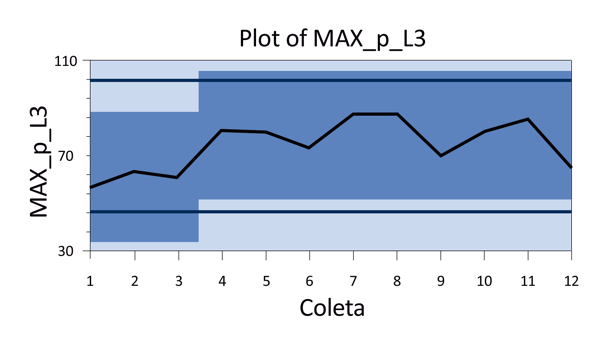
\includegraphics[width=0.45\textwidth]{imgs/lauracastilho22-image14.png}} \qquad
\subfloat[\label{laura-fig06-2}]{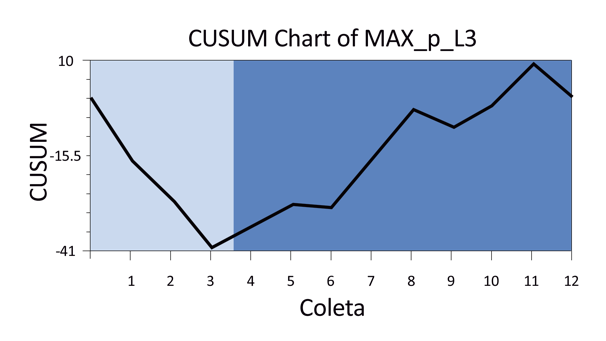
\includegraphics[width=0.45\textwidth]{imgs/lauracastilho22-image15.png}} \\
\caption{Change-point analyses of the maximums of [p] in French-L3.}
\label{laura-fig06}
\end{figure}

For [t], Level 1 phase shifts were also identified in the means and maximums,
occurring around Datapoint 4. For the means, the phase shift indicates an
increase in average from 33.44ms to 40.15ms, and in the maximums, from 58.91ms
to 70.33ms.

On the other hand, finally, we only found a significant phase shift in the
means of [k]. The Level 1 change was identified around Datapoint 6, indicating
an increase in average from 59.45ms to 66.26ms. Again, we reiterate the
subsystem's ability to change under the influence of changes in other
subsystems, especially the L2, since the new phases were always identified from
the beginning of the instruction period in that language.


%%%%%%%%%%%%%%%%%%%%%%%%%%%%%%%%%%%%%%%%%%%%%%%%%%%%%%%%%%%%%%%%%%%%%%
\section{Final Considerations}
We highlight the relevance of change-point analyses in verifying the emergence
of new developmental phases and we emphasize that change-point analyses allow
us to identify more than one change in each language subsystem, as shown in the
L2 data. Considering that changes in a multilingual system are constant and
that even attractor states are not permanent, an analysis of this sort provides
valuable information on the process of multilingual development. As shown in
our results, languages are entangled and interconnected in a multilingual
system, and they influence one another. Finally, we hope to contribute to the
area of language development in the light of Complex Dynamic Systems Theory.
Discussing methods of analysis that verify developmental changes is always
necessary. Specifically, change-point analyses help to identify the emergence
of new stages of development. As a non-linear process, we acknowledge the
fluctuations of the VOT values in the new developmental phase, as it probably
refers to a less strong attractor state, and even the emergence of a third
phase, different from both the initial phase and the phase under the influence
of the pedagogical intervention. These results show that language and learning
are constantly changing, demonstrating the relevance of an approach via CDST,
given that this, after all, constitutes a theory essentially about change.


%%%%%%%%%%%%%%%%%%%%%%%%%%%%%%%%%%%%%%%%%%%%%%%%%%%%%%%%%%%%%%%%%%%%%%
\bibliographystyle{plainnat}
\bibliography{lauracastilho22.bib}


